%Plantilla anteproyecto
%Última modificación: 21 de mayo de 2010
\documentclass[12pt,oneside,a4paper]{article}
\usepackage[spanish]{babel}
\usepackage[utf8]{inputenc}
\usepackage{graphicx}
\usepackage{amsmath}
\usepackage{amssymb}
\usepackage{color}
\usepackage{colortbl}
\usepackage{subfigure}
\usepackage{url}
\usepackage[all]{xy}
\linespread{1}
\setlength{\parskip}{1\baselineskip}
\parindent 1cm
\sloppy


%Opciones que debes descomentar mientras estemos revisando el anteproyecto
%\usepackage{lineno}
%\linenumbers
\usepackage[pagebackref=true,breaklinks=true,letterpaper=true,colorlinks,bookmarks=true]{hyperref}


%lista de palabras que Latex no parte bien
\hyphenation{pa-la-bras lis-ta}

\begin{document}

\thispagestyle{empty}

\begin{center}


Departamento de Teoría de la Señal y Comunicaciones\\
Escuela Politécnica Superior\\
Universidad de Alcalá\\

\vspace{1cm}


\includegraphics[width=4cm]{figuras/logo-uah.eps}

\textbf{ANTEPROYECTO}

\vspace{1cm}

\begin{large}\textbf{\textit{Sistema de adaptación inteligente de la velocidad para vehículos basados en inteligencia artificial y visión por computador}}\end{large}

\vfill

Diciembre - 2020

\end{center}

\begin{flushright}
\textit{Autor - \textbf{Sergio Sastre Arrojo}} \\
\textit{Director - \textbf{Roberto Javier López Sastre}}
\end{flushright}

\newpage
\section{Introducción}

En los últimos años, con la aparición de los sistemas ISA para conseguir que los vehículos adapten su velocidad se han evitado muchas desgracias afortunadamente. No obstante, han acarreado una serie de inconvenientes que se podrían mejorar. Por ejemplo: estos sistemas utilizan GPS, lo cual es muy eficiente para su propósito, pero en determinadas ocasiones (núcleos urbanos, distinción de carriles en una autovía con una carretera de servicio) pueden desembocar en situaciones de gran peligro.

¿Pero qué es un sistema ISA? ISA son las siglas de Intelligent Speed Adaptation, y como su propio nombre indica, es un sistema para adaptar la velocidad según diversos factores como adaptación por proximidad con otros vehículos u objetos, o por GPS como hemos mencionado anteriormente.

Es por ello que aquí presentamos una solución ante esos problemas: \[ISA^{2}\]

Con este nuevo sistema queremos adaptar la velocidad del vehículo en base a la situación del tráfico en cada momento.

La primera versión ya se realizó en su momento, por lo que el objetivo de este proyecto es mejorarlo a partir de nuevas tecnologías que han ido surgiendo en los últimos años \cite{isa2}.

\section{Objetivos y campos de aplicación}

Como ya hemos dicho, el objetivo principal de este proyecto es optimizar la primera versión que se hizo en su momento basándonos en la repetición de experimentos pasados para comprobar que funciona correctamente y de forma más eficiente que el anterior con un nuevo sistema de regresión y más componentes del proyecto que explicaremos más adelante.

Este proyecto será aplicable a cualquier campo relacionado con el automovilismo, para ayudar a mejorar la seguridad vial actual y, en esencia, para facilitar la lectura de la vía durante la conducción.

\section{Descripción del trabajo}

A continuación vamos a pasar a explicar las fases sobre las que se va a desarrollar el proyecto. Para ello nos ayudaremos de un diagrama de bloques:

\begin{center}
\xymatrix{*+[F]\txt{Modelos de predicción de segmentación semántica} \ar[r] & *+[F]\txt{Elaboración de sistema $ISA^2$} \\
*+[F]\txt{Preparación de experimentos para el sistema $ISA^2$} \ar[r] & *+[F]\txt{Repetición de experimentos anteriores}}
\end{center}
\subsection{Exploración de nuevos modelos de predicción de segmentación semántica}

Para esta fase investigaremos diferentes sistemas de predicción de segmentación semántica para que cuando el $ISA^2$ procese las imágenes, sepa diferenciar de la propia imagen qué es cada cosa de forma más eficiente que en la primera versión.
\subsection{Elaboración de sistema $ISA^2$}

Elaboraremos el nuevo sistema a partir del punto anterior para optimizarlo con respecto al anterior. Para ello pensaremos en nuevas técnicas de procesado de imagen y sistemas de regresión para su realización.
\subsection{Preparación de experimentos para el sistema $ISA^2$}

Para realizar esta fase, recabaremos múltiples imágenes de la vía en diferentes situaciones para tener un amplio rango de posibilidades a la hora de realizar los experimentos. Una vez hecho esto, las pasaremos por el sistema y comprobaremos su funcionamiento.

\subsection{Repetición de experimentos anteriores (de la primera versión) para el sistema $ISA^2$}

Por otro lado, tenemos una base de datos con imágenes de la vía que se utilizaron en la versión anterior. A partir de esas imágenes, realizaremos los mismo experimentos para comprobar la mejora del funcionamiento de este sistema con respecto al anterior.
%Ahora si, ¿cómo vas a hacer las cosas? Describe las partes, módulos o fases de tu proyecto, y añade un diagrama de bloques. Comenta cada uno de ellos, para que el lector entienda lo que persigues.

\section{Fases de desarrollo}

Teniendo en cuenta el apartado anterior, vamos a pasar a explicar de forma más detallada las diferentes fases del proyecto que antes hemos nombrado y descrito:

Dentro de este apartado vamos a tomar en cuenta el esquema utilizado en la versión 1.

\begin{figure}[h]
  \centering
  \includegraphics[width=4cm]{figuras/Figura_Esquema_ISA2_Version_1_SegSem.eps}
  \caption{$ISA^2$ Versión 1}
\end{figure}

\subsection{Exploración de nuevos modelos de predicción de segmentación semántica}

Como se puede ver en la figura anterior, el algoritmo que usamos en la primera versión se basa en una CNN (Convolutional Neural Network) desde la que le pasamos como input una imagen en diferentes escalas. Para esa versión se utilizó el modelo DeepLab como framework para hacer uso del algoritmo de segmentación semántica, teniendo como basa una CNN (en este caso, ResNet-101). De tal modo que la CNN calcula para cada una de las escalas el valor adecuado para los píxeles, para después fusionar los datos recogidos en cada escala.

Este proceso queremos mejorarlo en esta segunda versión: utilizando otros frameworks u otros modelos de CNN tal vez. O puede que mirándolo desde otro enfoque. Afortunadamente existe todo un baremo de posibilidades para optimizarlo\cite{segsem}. 
\subsection{Elaboración de sistema $ISA^2$}

Ya hemos explicado la parte referente al algoritmo de segmentación semántica, pero queda otra que es crucial para el proyecto: el sistema de regresión.
\subsubsection{Sistema de regresión}

Para esta parte vamos a seguir desde donde lo dejamos en el punto anterior: En la versión 1, tras la fusión de los datos en la CNN, recopilamos éstos en histogramas que informen de la frecuencia con la que han aparecido en la imagen los distintos objetos para saber qué porcentaje de imagen corresponde al paisaje, vehículos, etc,... 

Con todo ello construimos un descriptor de la imagen, el cual será pasado al sistema de regresión para que finalmente éste estime la velocidad adecuada para la imagen.

Los sistemas de regresión usados en la versión anterior, para los experimentos realizados, comprendían desde una ``regresión lineal'', hasta ``Lasso'' (Método de análisis de regresión) pasando por otros métodos como ``SVR'' (Support Vector Regression) o ``Boosting Trees''. Sin embargo, trabajaremos en otras aproximaciones basándonos, o bien en nuevas técnicas, o bien en lo ya usado en la versión anterior con un enfoque diferente. 
%Ahora debes detallar, de forma técnica, las fases de desarrollo. Te pongo un ejemplo.

%\begin{enumerate}
%\item Estudio de bibliografía y documentación sobre el problema de caza de pesca con gusano.
%\item \ldots
%\item Edición del manual de usuario de la aplicación.
%\item Edición del documento final utilizando \LaTeX.
%\end{enumerate}

%\section{Sobre \LaTeX}

%Si ya manejas \LaTeX no hace falta que leas esta sección.

%Necesitas aprender a manejar \LaTeX para escribir este anteproyecto y la memoria final del PFC. Verás que se trata de una herramienta estupenda para editar textos de forma profesional.

%La mejor manera de aprender es abrir un fichero \verb$.tex$ (por ejemplo el \verb$anteproyecto.tex$) y empezar a cambiar cosas en él y a compilarlo para generar un fichero \verb$.pdf$. Como editor te recomendamos Kile \cite{kile} (está en los repositorios de Ubuntu).

%Un página estupenda donde consultar dudas es esta \cite{wikibook}.

%Ya has visto que las citas bibliográficas (referencias a páginas web, artículos, congresos y libros) debes ponerlas utilizando el comando \verb$\cite$.

%Toda la bibliografía debes tenerla en un fichero \verb$.bib$ (en este caso estamos utilizando el fichero \verb$bibliografia-tfc.bib$). Se trata de un fichero que tiene la bibliografía en formato BibTex \cite{bibtex}. Para gestionar este fichero te recomendamos utilizar el programa JabRef \cite{jabref}. Si abres con JabRef el fichero \verb$bibliografia-tfc.bib$ verás las referencias que hemos utilizado en esta plantilla de anteproyecto. Tienes referencias a páginas web (que debes poner como tipo MISC) \cite{bibtex,jabref,wikibook}, a artículos de congresos (tipo INPROCEEDINGS) \cite{Lowe1999}, a artículos en revistas (tipo ARTICLE) \cite{Tuytelaars2008} y a libros (tipo BOOK) \cite{hartley2006}.

%Como ves, \LaTeX se encarga de numerar las referencias y de generar la bibliografía a partir del fichero \verb$.bib$.

%También puedes poner imágenes, como la representada en la Figura \ref{fig:ejemplo}. Recuerda utilizar \textbf{SÓLO} el formato \verb$.eps$ y compilar con latex (no con pdflatex). Para generar figuras en formato \verb$.eps$ te recomiendo utilizar el programa Inkscape\footnote{\url{http://www.inkscape.org/} -- también está en los repositorios de Ubuntu}. Por cierto, las notas a pie de página como esta debes tratar de no utilizarlas en exceso cuando escribas tu proyecto.

%\begin{figure}
 % \centering
  %
\includegraphics[width=4cm]{figuras/logo-uah.eps}
  %\caption{Un título.}
  %\label{fig:ejemplo}
%\end{figure}


%Bibliografía
\bibliographystyle{plain}
\bibliography{bibliografia-anteproyecto}


\end{document}
